\subsection{Schermata tests}
E' la schermata che mostra la lista di tutti i test presenti nel database.

\begin{figure}
\centering
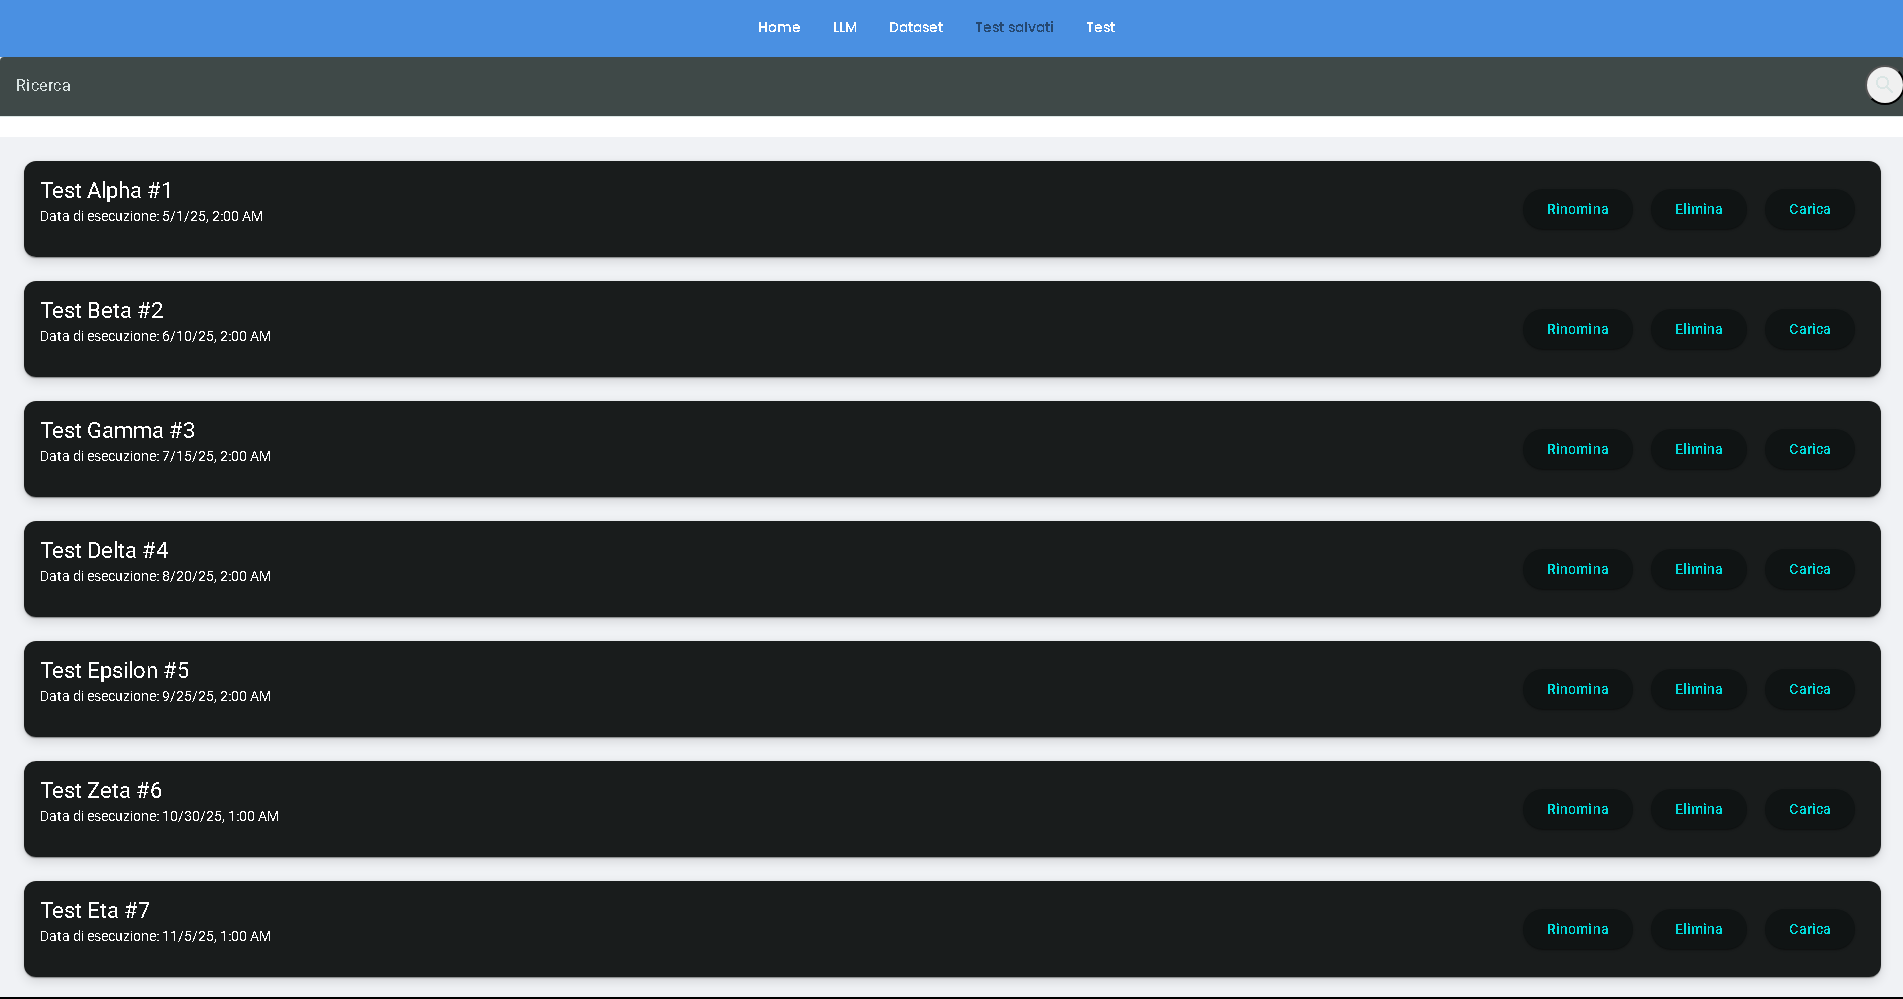
\includegraphics[width=0.25\linewidth]{Immagini/Test_Page.png}
\caption{\label{fig:tests}Schermata per la gestione dei test.}
\end{figure}

\subsubsection{Search Bar}
Permette un filtraggio preciso dei vari test caricati dal database.
\begin{figure}
\centering
\includegraphics[width=0.25\linewidth]{Immagini/SearchBar_Test_Option.png}
\caption{\label{fig:searchbar_test}Opzione per la ricerca dei test.}
\end{figure}

\subsubsection{Rename test button}
Consente di rinominare il test mostrando un form per l'inserimento del nuovo nome.
\begin{figure}
\centering
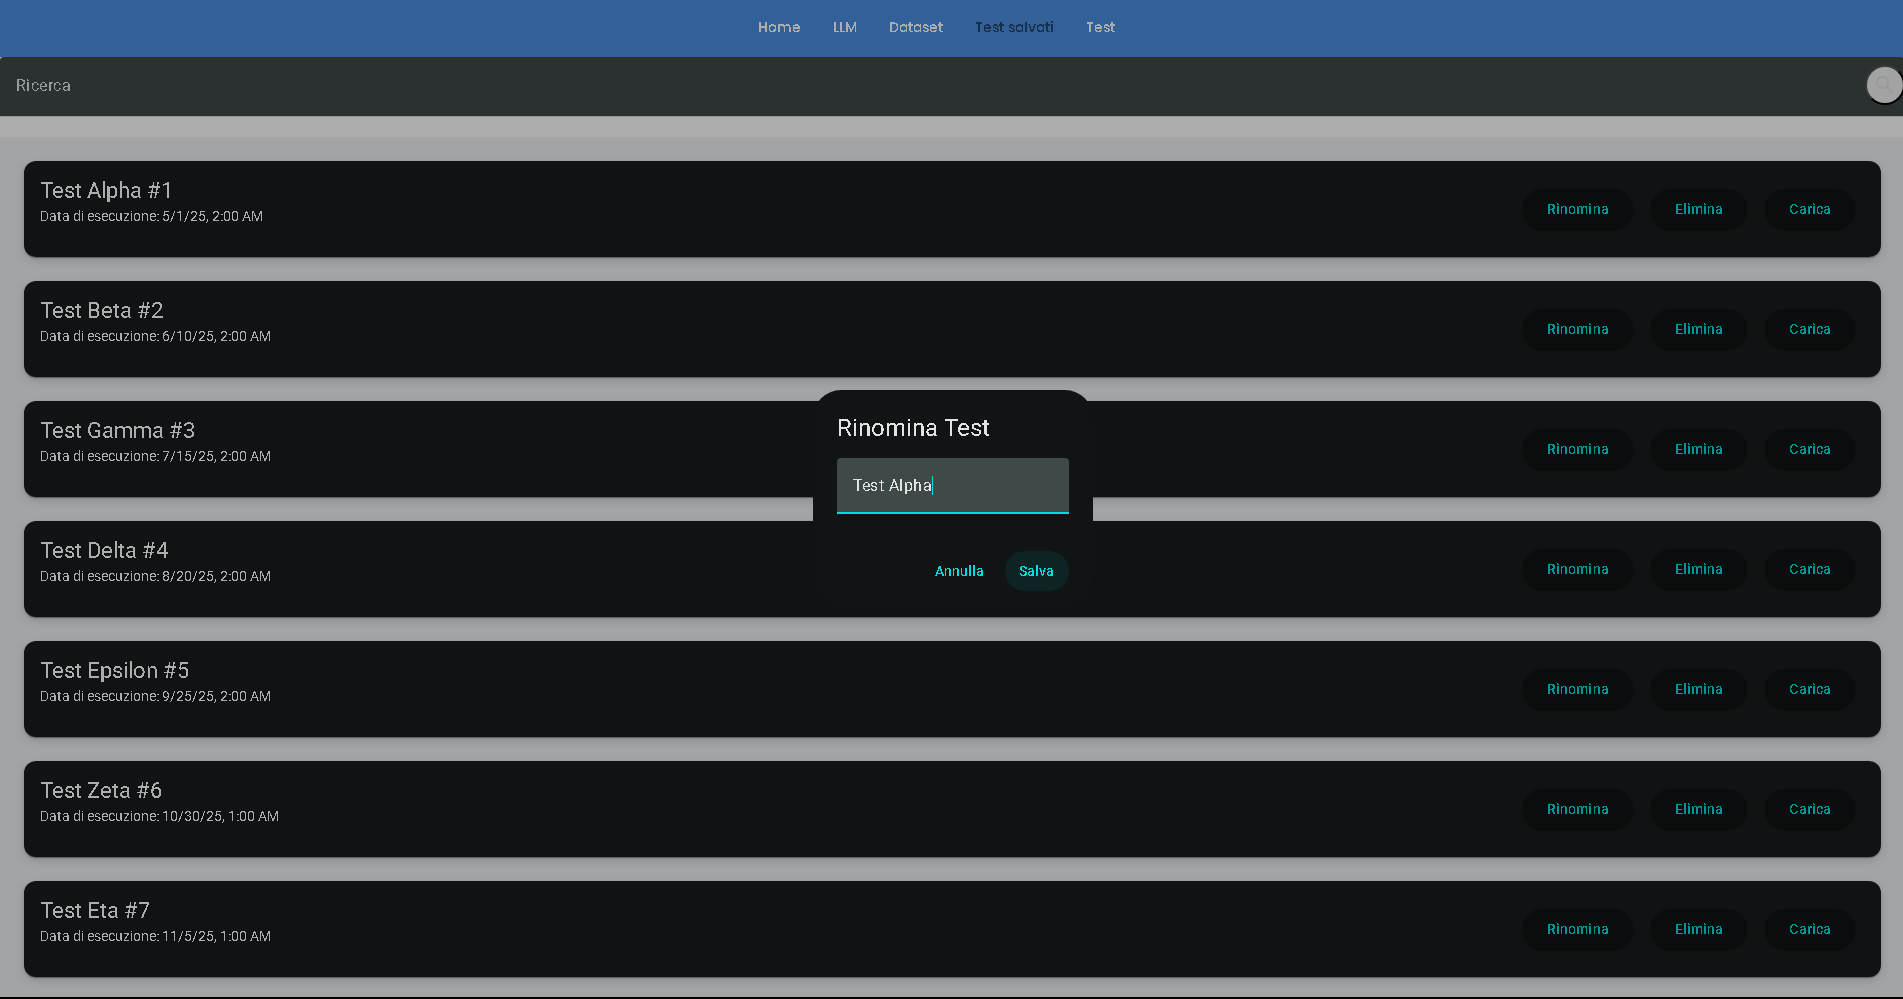
\includegraphics[width=0.25\linewidth]{Immagini/Rename_Test_Option.png}
\caption{\label{fig:rinomina_test}Opzione per la rinomina di un test.}
\end{figure}

\subsubsection{Delete test button}
Consente l'eliminazione dalla lista corrente e dal database del test.
\begin{figure}
\centering
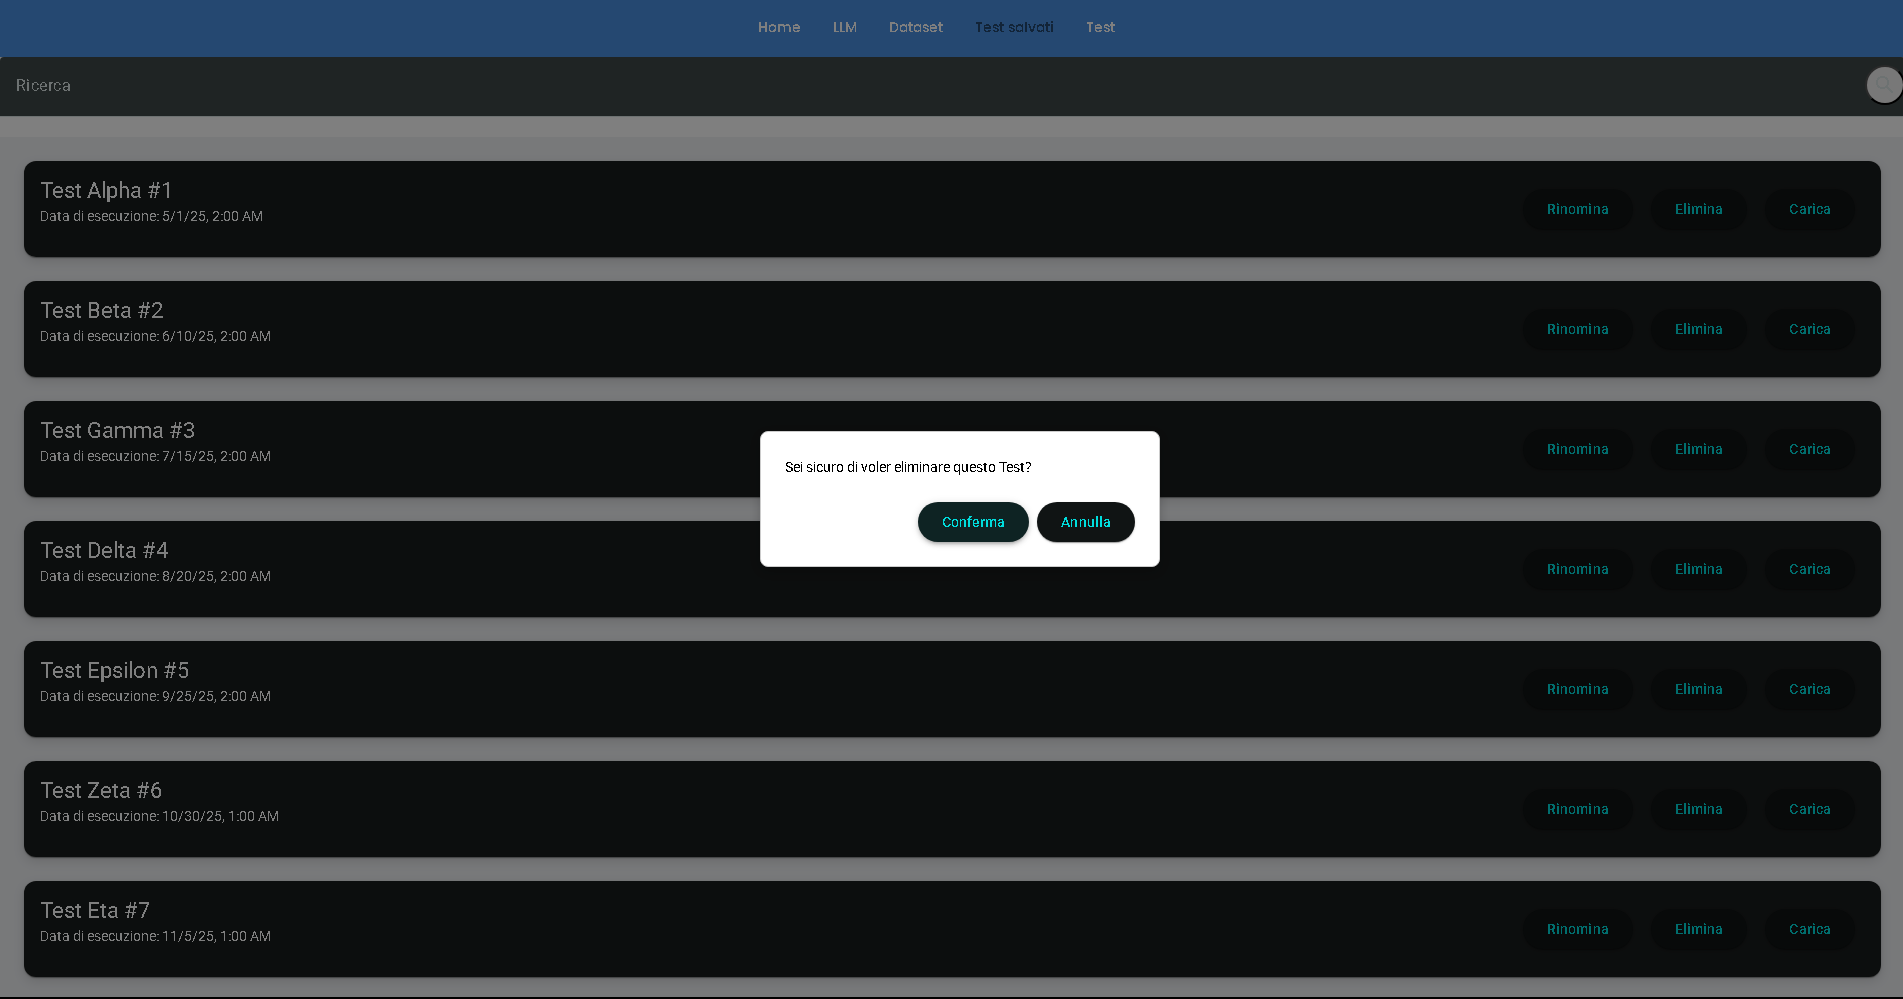
\includegraphics[width=0.25\linewidth]{Immagini/Delete_Test_Option.png}
\caption{\label{fig:eliminazione_test}Opzione per l'eliminazione di un test.}
\end{figure}

\subsubsection{Load test button}
Consente il caricamento in memoria del test, aprendo la pagina relativa al test con le informazioni relative.
\begin{figure}
\centering
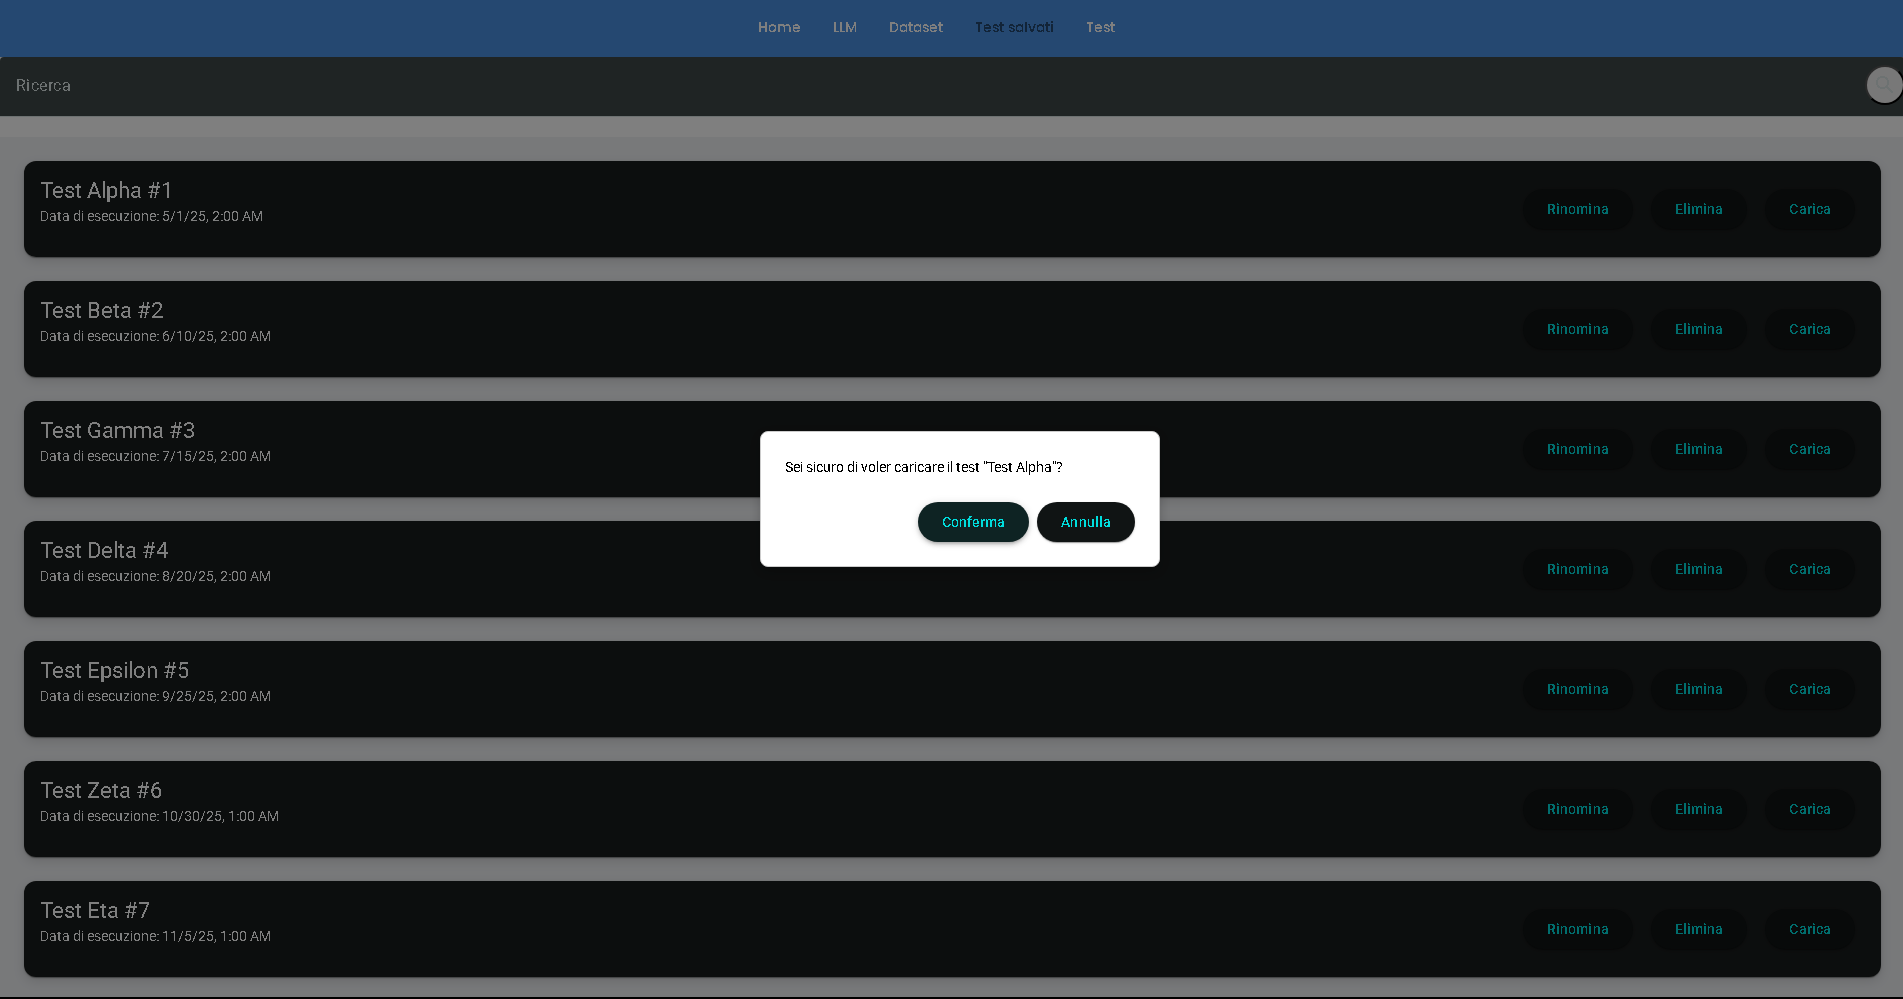
\includegraphics[width=0.25\linewidth]{Immagini/Load_Test_Option.png}
\caption{\label{fig:caricamento_test}Opzione per il caricamento di un test.}
\end{figure}